\documentclass[conference]{IEEEtran}
\usepackage{amsmath}
\usepackage{amsfonts}
\usepackage{listings}
\usepackage{graphicx}
\usepackage{hyperref}
\usepackage{karnaugh-map}
\usepackage{cite}

\def\BibTeX{{\rm B\kern-.05em{\sc i\kern-.025em b}\kern-.08em
    T\kern-.1667em\lower.7ex\hbox{E}\kern-.125emX}}

\title{Digital Clock using the Arduino Framework}
%with Multiplexing and Editing Features}

\author{
    \IEEEauthorblockN{Dhawal Saini and G. V. V. Sharma}
    \IEEEauthorblockA{Department of Electrical Engineering\\
    Indian Institute of Technology Hyderabad\\
    Email: gadepall@ee.iith.ac.in}
    %Email: ee24btech11015@iith.ac.in}
}

\begin{document}
\maketitle

% ---------------- Sections ----------------
\begin{abstract}
In this paper the design and implementation of a feature-rich digital clock is demonstrated. The system uses multiplexing to drive six seven-segment displays efficiently, minimizing I/O utilization. Key functionalities include timekeeping, digit-by-digit editing, and pause/play control. Boolean-based increment and decrement logic ensures more accurate cascading of seconds, minutes, and hours within standard constraints. The hardware setup, complemented by software debouncing and display refreshing, demonstrates a reliable, compact, and user-interactive digital clock suitable for both educational and practical applications.
\end{abstract}
\section{Introduction}
Digital timekeeping has long been a critical component of electronic system design, with classical digital design principles thoroughly discussed in foundational works such as \cite{mano2013digital, malvino2017digital, patterson2014computer}. The advent of microcontroller platforms, particularly Arduino, has enabled the development of compact, programmable clocks with enhanced user interactivity \cite{arduino_reference}. Techniques such as BCD-to-seven-segment interfacing and display multiplexing allow efficient utilization of limited I/O resources while maintaining accurate visual representation \cite{ti7447datasheet}. Inspired by these principles, a simple state machine representing a decade counter is  implemented in \cite{ddta}.  Based 
on this, 
we design an Arduino-based digital clock featuring six-digit multiplexed displays, pause/play functionality, and digit-by-digit editing with Boolean logic-driven increment and decrement operations.

%\begin{abstract}
In this paper the design and implementation of a feature-rich digital clock is demonstrated. The system uses multiplexing to drive six seven-segment displays efficiently, minimizing I/O utilization. Key functionalities include timekeeping, digit-by-digit editing, and pause/play control. Boolean-based increment and decrement logic ensures more accurate cascading of seconds, minutes, and hours within standard constraints. The hardware setup, complemented by software debouncing and display refreshing, demonstrates a reliable, compact, and user-interactive digital clock suitable for both educational and practical applications.
\end{abstract}

%\section{Introduction}
The digital clock system described here implements a feature-rich clock with editing capabilities using an Arduino microcontroller. The system utilizes a multiplexing technique to display time on six seven-segment displays using minimal I/O pins. This implementation includes pause/play functionality and digit-by-digit editing with increment and decrement buttons.

%\section{The Digital Clock}
\section{Clock Functionality and Hardware Setup}
Fig. \ref{fig:tinker}  shows the various hardware connections and the corresponding components are listed in 
Table \ref{tab:component}.  The clock follows the 23:59:59 format using 6 displays.  The first 2 represent hours, next 2 denote minutes and the last 2 count the seconds.

Pin connections from the Arduino to the four push buttons are available in 
Table \ref{tab:2.1}. Table \ref{tab:2.2} gives the connections between the Arduino and the IC 7447 display decoder.  The six displays are connected to the arduino through the pin connections listed in Table \ref{tab:2.3}.  Further, the pin connections for the IC 7447 to all the displays are available in Table \ref{tab:3}.
\begin{figure}[!ht]
\centering
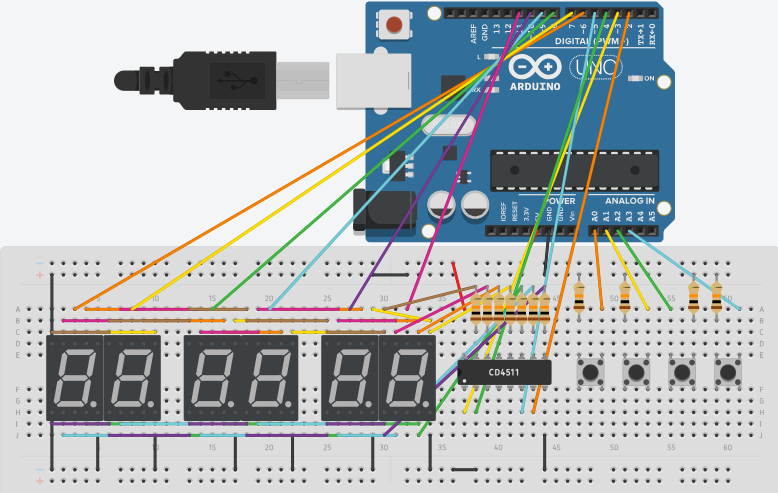
\includegraphics[width=\columnwidth]{figs/Clock_Tinkercad.png}
%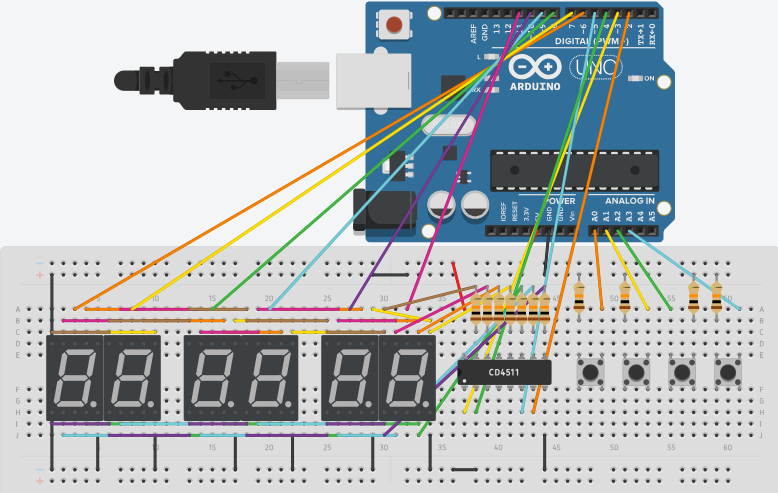
\includegraphics[width=0.45\textwidth]{figs/Clock_Tinkercad.png}
\caption{Tinkercad Simulation of the Digital Clock}
\label{fig:tinker}
\end{figure}
\begin{table}[!h]
\centering
\begin{tabular}{|l|c|c|}
\hline
Component & Value & Quantity\\
\hline
Arduino Uno & & 1\\
\hline
USB Cable & Type B & 1\\
\hline
Seven Segment Display & Common Cathode & 6\\
\hline
Push Buttons & & 4\\
\hline
IC 7447  &  & 1\\
\hline
Jumper Wires & M-M & 16\\
\hline
Breadboard & & 1\\
\hline
Resistors & 220$\Omega$ & 7\\
\hline
Resistors & 10$k\Omega$ (pull-down) & 4\\
\hline
\end{tabular}

\caption{Components List}
\label{tab:component}
\end{table}
\begin{table}[!h]
\centering
\centering
\begin{tabular}{|c|c|c|}
\hline
Button & Arduino Pin & Description\\
\hline
1 & D10 & Edit Mode Toggle\\
\hline
2 & D11 & Next Digit Selection\\
\hline
3 & D12  & Increment Digit\\
\hline
4 & D13  & Decrement Digit\\
\hline

\end{tabular}

\caption{Button to Arduino Connections}
\label{tab:2.1}
\end{table}
\begin{table}[!h]
\centering
\begin{tabular}{|c|c|c|}
\hline
IC 7447 PIN & Arduino Pin & Description\\
\hline

7 & D0 & BCD Bit 0 (A)\\
\hline
1 & D1 & BCD Bit 1 (B)\\
\hline
2 & D2 & BCD Bit 2 (C)\\
\hline
6 & D3 & BCD Bit 3 (D)\\
\hline
\end{tabular}

\caption{IC 7447 to Arduino Connections}
\label{tab:2.2}
\end{table}
\begin{table}[!h]
\centering
\begin{tabular}{|c|c|c|}
\hline
Display & Arduino Pin & Description\\
\hline
1  & D4 & Hours Tens Digit\\
\hline
2  & D5 & Hours Units Digit\\
\hline
3  & D6 & Minutes Tens Digit\\
\hline
4  & D7 & Minutes Units Digit\\
\hline
5 & D8 & Seconds Tens Digit\\
\hline
6  & D9 & Seconds Units Digit\\
\hline
\end{tabular}

\caption{Display to Arduino Connections}
\label{tab:2.3}
\end{table}
\begin{table}[!h]
\centering
\begin{tabular}{|c|c|c|}
\hline
IC 7447 & Seven Segment (All)\\
\hline
13 & a\\
\hline
12 & b\\
\hline
11 & c\\
\hline
10 & d\\
\hline
9 & e\\
\hline
15 & f\\
\hline
14 & g\\
\hline
8 & Ground\\
\hline
16 & 5V \\
\hline
\end{tabular}

\caption{BCD to 7-Segment Connections}
\label{tab:3}
\end{table}
\section{Clock Logic}
%\section{Components}
\centering
\begin{tabular}{|l|c|c|}
\hline
Component & Value & Quantity\\
\hline
Arduino Uno & & 1\\
\hline
USB Cable & Type B & 1\\
\hline
Seven Segment Display & Common Cathode & 6\\
\hline
Push Buttons & & 4\\
\hline
IC 7447  &  & 1\\
\hline
Jumper Wires & M-M & 16\\
\hline
Breadboard & & 1\\
\hline
Resistors & 220$\Omega$ & 7\\
\hline
Resistors & 10$k\Omega$ (pull-down) & 4\\
\hline
\end{tabular}\\
\centerline{Table 1.0: Components List}


%\section{Circuit Connections}
\raggedright
Make the connections to the devices as per the tables below.
\begin{centering}
\subsection{Button connections to Arduino}
\end{centering}
\raggedright
The buttons and displays are arranged chronologically from left to right.\\
\vspace{0.25cm}
\centering
\begin{tabular}{|c|c|c|}
\hline
Button & Arduino Pin & Description\\
\hline
1 & D10 & Edit Mode Toggle\\
\hline
2 & D11 & Next Digit Selection\\
\hline
3 & D12  & Increment Digit\\
\hline
4 & D13  & Decrement Digit\\
\hline

\end{tabular}\\
\centerline{Table 2.1: Button to Arduino Connections}


\subsection{IC 7447 connections to Arduino}
\raggedright
\vspace{0.25cm}
\centering
\begin{tabular}{|c|c|c|}
\hline
IC 7447 PIN & Arduino Pin & Description\\
\hline

7 & D0 & BCD Bit 0 (A)\\
\hline
1 & D1 & BCD Bit 1 (B)\\
\hline
2 & D2 & BCD Bit 2 (C)\\
\hline
6 & D3 & BCD Bit 3 (D)\\
\hline
\end{tabular}\\
\centerline{Table 2.2: IC 7447 to Arduino Connections}


\subsection{Display connections to Arduino}
\raggedright
The digital pins are connected to COM of displays.\\
\vspace{0.25cm}
\centering
\begin{tabular}{|c|c|c|}
\hline
Display & Arduino Pin & Description\\
\hline
1  & D4 & Hours Tens Digit\\
\hline
2  & D5 & Hours Units Digit\\
\hline
3  & D6 & Minutes Tens Digit\\
\hline
4  & D7 & Minutes Units Digit\\
\hline
5 & D8 & Seconds Tens Digit\\
\hline
6  & D9 & Seconds Units Digit\\
\hline
\end{tabular}\\
\centerline{Table 2.3: Display to Arduino Connections}


\subsection{Connections from Seven Segment to BCD}
\raggedright
Make the seven-segment connections identical for all seven\\ \raggedright segments. In total, there should only be 7 wires of output\\ \raggedright coming from the seven-segment display array.\\
\vspace{0.25cm}
\centering
\begin{tabular}{|c|c|c|}
\hline
IC 7447 & Seven Segment (All) & Name\\
\hline
Pin 13 & a & Controls segment a\\
\hline
Pin 12 & b & Controls segment b\\
\hline
Pin 11 & c & Controls segment c\\
\hline
Pin 10 & d & Controls segment d\\
\hline
Pin 9 & e & Controls segment e\\
\hline
Pin 15 & f & Controls segment f\\
\hline
Pin 14 & g & Controls segment g\\
\hline
Pin 8 & Ground & Ground Supply\\
\hline
Pin 16 & 5V & Power Supply\\
\hline
\end{tabular}\\
\centerline{Table 3.0: BCD to 7-Segment Connections}


\section{Constraints Explanation}
\begin{itemize}
    \item \textbf{Seconds and Minutes Ones:} 0–9, standard BCD.
    \item \textbf{Seconds and Minutes Tens:} 0–5, to match 0–59 range.
    \item \textbf{Hours Ones:} 0–9 if hours tens = 0 or 1, but 0–3 if hours tens = 2, ensuring 24-hour format.
    \item \textbf{Hours Tens:} 0–2.
\end{itemize}


%\section{Increment Logic and Truth Tables}

%\subsection{Seconds Ones (0-9)}
\subsection{Displays 2 (Display1 $\ne 2$), 4 and 6}
The truth table is available in 
Table 
\ref{tab:4}
and the corresponding K-maps using dont cares for the output variables are given in 
Figs. \ref{fig:kmapA-4-6}-\ref{fig:kmapD-4-6} yielding the following logic equations.
\begin{align}
    A &= W_1' \\
    B &= (W_1 X_1' Z_1') + (W_1' X_1) \\
    C &= (X_1' Y_1) + (W_1' Y_1) + (W_1 X_1 Y_1') \\
    D &= (W_1' Z_1) + (W_1 X_1 Y_1) 
\end{align}
\begin{table}[!h]
\centering
\begin{tabular}{|c|c|c|c||c|c|c|c|}
\hline
Z & Y & X & W & D & C & B & A\\
\hline
0 & 0 & 0 & 0 & 0 & 0 & 0 & 1\\
0 & 0 & 0 & 1 & 0 & 0 & 1 & 0\\
0 & 0 & 1 & 0 & 0 & 0 & 1 & 1\\
0 & 0 & 1 & 1 & 0 & 1 & 0 & 0\\
0 & 1 & 0 & 0 & 0 & 1 & 0 & 1\\
0 & 1 & 0 & 1 & 0 & 1 & 1 & 0\\
0 & 1 & 1 & 0 & 0 & 1 & 1 & 1\\
0 & 1 & 1 & 1 & 1 & 0 & 0 & 0\\
1 & 0 & 0 & 0 & 1 & 0 & 0 & 1\\
1 & 0 & 0 & 1 & 0 & 0 & 0 & 0\\
\hline
\end{tabular}

\caption{}
\label{tab:4}
\end{table}

\begin{figure}[!h]
    \centering
\begin{karnaugh-map}[4][4][1][][]
    \maxterms{1,3,5,7,9}
    \minterms{0,2,4,6,8}
    \indeterminants{10,11,12,13,14,15}

    \implicantedge{0}{8}{2}{10}
    \draw[color=black, ultra thin] (0, 4) --
        node [pos=0.7, above right, anchor=south west] {$XW$}
        node [pos=0.7, below left, anchor=north east] {$ZY$} 
        ++(135:1);
\end{karnaugh-map}
\caption{A}
\label{fig:kmapA-4-6}
\end{figure}
\begin{figure}[!h]
    \centering
\begin{karnaugh-map}[4][4][1][][]
    \minterms{1,2,5,6}
    \maxterms{0,3,4,7,8,9}
    \indeterminants{10,11,12,13,14,15}

    \implicant{1}{5}
    \implicant{2}{10}

    \draw[color=black, ultra thin] (0, 4) --
        node [pos=0.7, above right, anchor=south west] {$XW$}
        node [pos=0.7, below left, anchor=north east] {$ZY$} 
        ++(135:1);
\end{karnaugh-map}
\caption{B}
\label{fig:kmapB-4-6}
\end{figure}
\begin{figure}[!h]
    \centering

\begin{karnaugh-map}[4][4][1][][]
    \minterms{3,4,5,6}
    \maxterms{0,1,2,7,8,9}
    \indeterminants{10,11,12,13,14,15}

    \implicant{4}{5}    
    \implicant{3}{3}
    \implicantedge{4}{4}{6}{6}   

    \draw[color=black, ultra thin] (0, 4) --
        node [pos=0.7, above right, anchor=south west] {$XW$}
        node [pos=0.7, below left, anchor=north east] {$ZY$} 
        ++(135:1);
\end{karnaugh-map}
\caption{C}
\label{fig:kmapC-4-6}
\end{figure}
\begin{figure}
	\centering
\begin{karnaugh-map}[4][4][1][][]
    \minterms{7,8}
    \maxterms{0,1,2,3,4,6,5,9}
    \indeterminants{10,11,12,13,14,15}

    \implicant{7}{15}    
    \implicantedge{12}{8}{14}{10}   

    \draw[color=black, ultra thin] (0, 4) --
        node [pos=0.7, above right, anchor=south west] {$XW$}
        node [pos=0.7, below left, anchor=north east] {$ZY$} 
        ++(135:1);
\end{karnaugh-map}
\caption{D}
\label{fig:kmapD-4-6}
\end{figure}
\subsection{Displays 3 and 5}
The truth table is available in 
Table 
\ref{tab:5}
and the corresponding K-maps using dont cares for the output variables are given in 
Figs. \ref{fig:kmapA-3-5}-\ref{fig:kmapC-3-5} yielding the following logic equations.
\begin{align}
    A &= W_2' \\
    B &= (W_2 X_2' Y_2') + (W_2' X_2) \\
    C &= (W_2 X_2) + (W_2' X_2' Y_2) \\
    D &= 0 \\
\end{align}
\begin{table}[!h]
\centering
\begin{tabular}{|c|c|c|c||c|c|c|c|}
\hline
Z & Y & X & W & D & C & B & A\\
\hline
0 & 0 & 0 & 0 & 0 & 0 & 0 & 1\\
0 & 0 & 0 & 1 & 0 & 0 & 1 & 0\\
0 & 0 & 1 & 0 & 0 & 0 & 1 & 1\\
0 & 0 & 1 & 1 & 0 & 1 & 0 & 0\\
0 & 1 & 0 & 0 & 0 & 1 & 0 & 1\\
0 & 1 & 0 & 1 & 0 & 0 & 0 & 0\\
\hline
\end{tabular}

\caption{}
\label{tab:5}
\end{table}
\begin{figure}
	\centering
\begin{karnaugh-map}[4][4][1][][]
    \maxterms{1,3,5}
    \minterms{0,2,4}
    \indeterminants{6,7,8,9,10,11,12,13,14,15}

    \implicantedge{0}{8}{2}{10}
    \draw[color=black, ultra thin] (0, 4) --
        node [pos=0.7, above right, anchor=south west] {$XW$}
        node [pos=0.7, below left, anchor=north east] {$ZY$} 
        ++(135:1);
\end{karnaugh-map}
\caption{A}
\label{fig:kmapA-3-5}
\end{figure}

\begin{figure}
	\centering
\begin{karnaugh-map}[4][4][1][][]
    \maxterms{0,4,3,5}
    \minterms{1,2}
    \indeterminants{6,7,8,9,10,11,12,13,14,15}

    \implicant{2}{10}
    \implicantedge{1}{1}{9}{9}

    \draw[color=black, ultra thin] (0, 4) --
        node [pos=0.7, above right, anchor=south west] {$XW$}
        node [pos=0.7, below left, anchor=north east] {$ZY$} 
        ++(135:1);
\end{karnaugh-map}
\caption{B}
\label{fig:kmapB-3-5}
\end{figure}

\begin{figure}
	\centering
\begin{karnaugh-map}[4][4][1][][]
    \maxterms{0,1,2,5}
    \minterms{3,4}
    \indeterminants{6,7,8,9,10,11,12,13,14,15}

    \implicant{4}{8}
    \implicant{3}{11}

    \draw[color=black, ultra thin] (0, 4) --
        node [pos=0.7, above right, anchor=south west] {$XW$}
        node [pos=0.7, below left, anchor=north east] {$ZY$} 
        ++(135:1);
\end{karnaugh-map}
\caption{C}
\label{fig:kmapC-3-5}
\end{figure}
\subsection{Display 2 (Display1 = 2)}
The truth table is available in 
Table 
\ref{tab:6}
and the corresponding K-maps using dont cares for the output variables are given in 
Figs. \ref{fig:kmapA-2}-\ref{fig:kmapB-2} yielding the following logic equations.
\begin{table}[!h]
\centering
\begin{tabular}{|c|c||c|c|c|c|}
\hline
X & W & D & C & B & A\\
\hline
0 & 0 & 0 & 0 & 0 & 1\\
0 & 1 & 0 & 0 & 1 & 0\\
1 & 0 & 0 & 0 & 1 & 1\\
1 & 1 & 0 & 0 & 0 & 0\\
\hline
\end{tabular}


\caption{}
\label{tab:6}
\end{table}
\begin{figure}
	\centering
\begin{karnaugh-map}[2][2][1][][]
    \minterms{0,2}
    \maxterms{3,1}

    \implicant{0}{2}
    \draw[color=black, ultra thin] (0, 2) --
        node [pos=0.7, above right, anchor=south west] {$W$}
        node [pos=0.7, below left, anchor=north east] {$X$} 
        ++(135:1);
\end{karnaugh-map}
\caption{A}
\label{fig:kmapA-2}
\end{figure}

\begin{figure}
	\centering
\begin{karnaugh-map}[2][2][1][][]
    \minterms{1,2}
    \maxterms{3,0}
    \implicant{1}{1}
    \implicant{2}{2}
    \draw[color=black, ultra thin] (0, 2) --
        node [pos=0.7, above right, anchor=south west] {$W$}
        node [pos=0.7, below left, anchor=north east] {$X$} 
        ++(135:1);
\end{karnaugh-map}
\caption{B}
\label{fig:kmapB-2}
\end{figure}
\begin{align}
    A &= W_5' \\
    B &= (W_5 X_5') + (W_5' X_5) \\
    C &= 0 \\
    D &= 0 
\end{align}
%
\subsection{Hours Tens (0-2)}
\begin{center}
\begin{tabular}{|c|c||c|c|c|c|}
\hline
X & W & D & C & B & A\\
\hline
0 & 0 & 0 & 0 & 0 & 1\\
0 & 1 & 0 & 0 & 1 & 0\\
1 & 0 & 0 & 0 & 0 & 0\\
\hline
\end{tabular}
\end{center}


\begin{karnaugh-map}[2][2][1][][]
    \minterms{0}
    \maxterms{2,1}
    \indeterminants{3}

    \implicant{0}{0}
    \draw[color=black, ultra thin] (0, 2) --
        node [pos=0.7, above right, anchor=south west] {$W$}
        node [pos=0.7, below left, anchor=north east] {$X$} 
        ++(135:1);
\end{karnaugh-map}
\begin{align}
    A &= W_6' X_6' \notag
\end{align}

\begin{karnaugh-map}[2][2][1][][]
    \minterms{1}
    \maxterms{2,0}
    \indeterminants{3}

    \implicant{1}{1}
    \draw[color=black, ultra thin] (0, 2) --
        node [pos=0.7, above right, anchor=south west] {$W$}
        node [pos=0.7, below left, anchor=north east] {$X$} 
        ++(135:1);
\end{karnaugh-map}
\begin{align}
    B &= W_6 X_6' \notag
\end{align}

\begin{align}
    C &= 0 \notag\\
    D &= 0 \notag
\end{align}

\section{Decrement Logic}

\subsection{Seconds Ones (0-9)}
\begin{center}
\begin{tabular}{|c|c|c|c||c|c|c|c|}
\hline
Z & Y & X & W & D & C & B & A\\
\hline
0 & 0 & 0 & 0 & 1 & 0 & 0 & 1\\
0 & 0 & 0 & 1 & 0 & 0 & 0 & 0\\
0 & 0 & 1 & 0 & 0 & 0 & 0 & 1\\
0 & 0 & 1 & 1 & 0 & 0 & 1 & 0\\
0 & 1 & 0 & 0 & 0 & 0 & 1 & 1\\
0 & 1 & 0 & 1 & 0 & 1 & 0 & 0\\
0 & 1 & 1 & 0 & 0 & 1 & 0 & 1\\
0 & 1 & 1 & 1 & 0 & 1 & 1 & 0\\
1 & 0 & 0 & 0 & 0 & 1 & 1 & 1\\
1 & 0 & 0 & 1 & 1 & 0 & 0 & 0\\
\hline
\end{tabular}
\end{center}


\begin{karnaugh-map}[4][4][1][][]
    \minterms{0,2,4,6,8}
    \maxterms{1,3,5,7,9}
    \indeterminants{10,11,12,13,14,15}

    \implicantedge{0}{8}{2}{10}
    \draw[color=black, ultra thin] (0, 4) --
        node [pos=0.7, above right, anchor=south west] {$XW$}
        node [pos=0.7, below left, anchor=north east] {$ZY$} 
        ++(135:1);
\end{karnaugh-map}
\begin{align}
    A &= W_1' \notag
\end{align}

\begin{karnaugh-map}[4][4][1][][]
    \minterms{3,4,7,8}
    \maxterms{0,1,2,5,6,9}
    \indeterminants{10,11,12,13,14,15}

    \implicant{3}{7}
    \implicant{4}{4}
    \implicant{8}{8}
    
    \draw[color=black, ultra thin] (0, 4) --
        node [pos=0.7, above right, anchor=south west] {$XW$}
        node [pos=0.7, below left, anchor=north east] {$ZY$} 
        ++(135:1);
\end{karnaugh-map}
\begin{align}
    B &= (X_1' W_1' ((Z_1' Y_1) + (Z_1 Y_1'))) + (Z_1' W_1 X_1) \notag
\end{align}

\begin{karnaugh-map}[4][4][1][][]
    \minterms{5,6,7,8}
    \maxterms{0,1,2,3,4,9}
    \indeterminants{10,11,12,13,14,15}

    \implicant{5}{7}
    \implicant{7}{6}
    \implicant{8}{8}
    \draw[color=black, ultra thin] (0, 4) --
        node [pos=0.7, above right, anchor=south west] {$XW$}
        node [pos=0.7, below left, anchor=north east] {$ZY$} 
        ++(135:1);
\end{karnaugh-map}
\begin{align}
    C &= (Z_1' Y_1 (X_1 + W_1)) + (Z_1 X_1' W_1' Y_1') \notag
\end{align}

\begin{karnaugh-map}[4][4][1][][]
    \minterms{0,9}
    \maxterms{1,2,3,4,5,6,7,8}
    \indeterminants{10,11,12,13,14,15}

    \implicant{0}{0}
    \implicant{9}{9}
    \draw[color=black, ultra thin] (0, 4) --
        node [pos=0.7, above right, anchor=south west] {$XW$}
        node [pos=0.7, below left, anchor=north east] {$ZY$} 
        ++(135:1);
\end{karnaugh-map}
\begin{align}
    D &= X_1' Y_1' ((Z_1 W_1) + (Z_1' W_1')) \notag
\end{align}

\subsection{Seconds Tens (0-5)}
\begin{center}
\begin{tabular}{|c|c|c|c||c|c|c|c|}
\hline
Z & Y & X & W & D & C & B & A\\
\hline
0 & 0 & 0 & 0 & 0 & 1 & 0 & 1\\
0 & 0 & 0 & 1 & 0 & 0 & 0 & 0\\
0 & 0 & 1 & 0 & 0 & 0 & 0 & 1\\
0 & 0 & 1 & 1 & 0 & 0 & 1 & 0\\
0 & 1 & 0 & 0 & 0 & 0 & 1 & 1\\
0 & 1 & 0 & 1 & 0 & 1 & 0 & 0\\
\hline
\end{tabular}
\end{center}


\begin{karnaugh-map}[4][4][1][][]
    \minterms{0,2,4}
    \maxterms{1,3,5}
    \indeterminants{6,7,8,9,10,11,12,13,14,15}

    \implicantedge{0}{8}{2}{10}
    \draw[color=black, ultra thin] (0, 4) --
        node [pos=0.7, above right, anchor=south west] {$XW$}
        node [pos=0.7, below left, anchor=north east] {$ZY$} 
        ++(135:1);
\end{karnaugh-map}
\begin{align}
    A &= W_2' \notag
\end{align}

\begin{karnaugh-map}[4][4][1][][]
    \minterms{3,4}
    \maxterms{0,1,2,5}
    \indeterminants{6,7,8,9,10,11,12,13,14,15}

    \implicantedge{3}{3}{11}{11}
    \implicant{4}{12}

    \draw[color=black, ultra thin] (0, 4) --
        node [pos=0.7, above right, anchor=south west] {$XW$}
        node [pos=0.7, below left, anchor=north east] {$ZY$} 
        ++(135:1);
\end{karnaugh-map}
\begin{align}
    B &= (Y_2 X_2' W_2') + (Y_2' X_2 W_2) \notag
\end{align}

\begin{karnaugh-map}[4][4][1][][]
    \minterms{0,5}
    \maxterms{4,1,2,3}
    \indeterminants{6,7,8,9,10,11,12,13,14,15}

    \implicantedge{0}{0}{8}{8}
    \implicant{5}{13}

    \draw[color=black, ultra thin] (0, 4) --
        node [pos=0.7, above right, anchor=south west] {$XW$}
        node [pos=0.7, below left, anchor=north east] {$ZY$} 
        ++(135:1);
\end{karnaugh-map}
\begin{align}
    C &= X_2' ((Y_2 W_2) + (Y_2' W_2')) \notag
\end{align}

\begin{align}
    D &= 0 \notag
\end{align}

\subsection{Minutes Ones (0-9)}
\textit{Same as Seconds Ones with W3/X3/Y3/Z3.}

\subsection{Minutes Tens (0-5)}
\textit{Same as Seconds Tens with W4/X4/Y4/Z4.}

\subsection{Hours Ones }
\textbf{I. Tens = 0/1 → 0-9 }\\
\textit{Same as Seconds Ones with W5/X5/Y5/Z5.}

\textbf{II. Tens = 2 → 0-3 }
\begin{tabular}{|c|c||c|c|c|c|}
\hline
X & W & D & C & B & A\\
\hline
0 & 0 & 0 & 0 & 1 & 1\\
0 & 1 & 0 & 0 & 0 & 0\\
1 & 0 & 0 & 0 & 0 & 1\\
1 & 1 & 0 & 0 & 1 & 0\\
\hline
\end{tabular}


\begin{karnaugh-map}[2][2][1][][]
    \minterms{0,2}
    \maxterms{1,3}

    \implicant{0}{2}
    \draw[color=black, ultra thin] (0, 2) --
        node [pos=0.7, above right, anchor=south west] {$W$}
        node [pos=0.7, below left, anchor=north east] {$X$} 
        ++(135:1);
\end{karnaugh-map}
\begin{align}
    A &= W_5' \notag
\end{align}

\begin{karnaugh-map}[2][2][1][][]
    \minterms{0,3}
    \maxterms{1,2}

    \implicant{0}{0}
    \implicant{3}{3}

    \draw[color=black, ultra thin] (0, 2) --
        node [pos=0.7, above right, anchor=south west] {$W$}
        node [pos=0.7, below left, anchor=north east] {$X$} 
        ++(135:1);
\end{karnaugh-map}
\begin{align}
    B &= (X_5 W_5) + (X_5' W_5') \notag
\end{align}

\begin{align}
    C &= 0 \notag\\
    D &= 0 \notag
\end{align}

\subsection{Hours Tens (0-2)}
\begin{center}
\begin{tabular}{|c|c||c|c|c|c|}
\hline
X & W & D & C & B & A\\
\hline
0 & 0 & 0 & 0 & 1 & 0\\
0 & 1 & 0 & 0 & 0 & 0\\
1 & 0 & 0 & 0 & 0 & 1\\
\hline
\end{tabular}
\end{center}


\begin{karnaugh-map}[2][2][1][][]
    \minterms{2}
    \maxterms{0,1}
    \indeterminants{3}

    \implicant{2}{2}
    \draw[color=black, ultra thin] (0, 2) --
        node [pos=0.7, above right, anchor=south west] {$W$}
        node [pos=0.7, below left, anchor=north east] {$X$} 
        ++(135:1);
\end{karnaugh-map}
\begin{align}
    A &= X_6 W_6' \notag
\end{align}

\begin{karnaugh-map}[2][2][1][][]
    \minterms{0}
    \maxterms{2,1}
    \indeterminants{3}

    \implicant{0}{0}
    \draw[color=black, ultra thin] (0, 2) --
        node [pos=0.7, above right, anchor=south west] {$W$}
        node [pos=0.7, below left, anchor=north east] {$X$} 
        ++(135:1);
\end{karnaugh-map}
\begin{align}
    B &= X_6' W_6' \notag
\end{align}

\begin{align}
    C &= 0 \notag\\
    D &= 0 \notag
\end{align}







\subsection{Multiplexing Technique}
All BCD inputs (A-D) are shared among six seven-segment displays. Displays are enabled one at a time using EN[0..5] = D4-D9 (see Table \ref{tab:2.3}). Each digit is displayed for 1ms, creating a fast alternating effect that appears continuous. This saves I/O pins and allows full six-digit display.



\section{Digit Editing Logic}
The clock allows pausing and digit-by-digit editing:

\begin{enumerate}
    \item Press PAUSE (D10) to toggle run/edit mode. In edit mode, the clock stops.
    \item Press NEXT (D11) to select the digit to edit (cycles 0-5: sec1, sec10, min1, min10, hr1, hr10).
    \item Press INC (D12) to increment the selected digit with rollovers.
    \item Press DEC (D13) to decrement the selected digit with rollunders.
    \item Selected digit blinks every 500ms to indicate focus.
\end{enumerate}


\subsection{Implementation}
    Pressing Button 1 toggles between run mode and edit mode. In edit mode, the clock pauses.  Following functions are available in edit mode.
    The selected digit blinks at 5Hz (200ms on, 200ms off) for visual feedback.
\begin{enumerate}
    \item Pressing Button 2 selects the next digit for editing (cycles through all six digits).
    \item Pressing Button 3 increments the currently selected digit using the increment logic tables.
    \item Pressing Button 4 decrements the currently selected digit using the decrement logic tables.
\end{enumerate}

Following are the steps to upload code to the Arduino
\begin{enumerate}
    \item Connect Arduino to computer via USB
    \item Upload the following code to the Arduino 
	    %using PlatformIO.
	%{\em Platformio}.
\fbox{\parbox{\linewidth}{\url{https://github.com/gadepall/clock/blob/main/codes/code.cpp}
}}
%\item Open PlatformIO, select New Project and then fill in the details (name, board \& framework).
%\item Then replace contents in src/main.cpp with the above code, now run \& upload that code to Arduino Uno.
\end{enumerate}
The Arduino code implements
\begin{itemize}
    \item Timer interrupt for clock ticking (10Hz interrupt rate)
    \item Button debouncing with software delays
    \item Multiplexed display refresh
    \item Editing mode with digit selection and value modification using the Boolean logic from the tables
    \item Proper constraints on time values (hours 0-23, minutes 0-59, seconds 0-59)
\end{itemize}

\section{Execution}
\subsection{Upload Code to Arduino}
\begin{enumerate}
    \item Connect Arduino to computer via USB
    \item Upload the following code to the Arduino using PlatformIO.
	%{\em Platformio}.
\fbox{\parbox{\linewidth}{\url{https://github.com/gadepall/clock/blob/main/codes/code.cpp}
}}
\item Open PlatformIO, select New Project and then fill in the details (name, board \& framework).
\item Then replace contents in src/main.cpp with the above code, now run \& upload that code to Arduino Uno.
\end{enumerate}

\subsection{Hardware Build}
\begin{enumerate}
    \item Connect the seven-segment displays to the breadboard
    \item Connect all segment outputs together (through resistors)
    \item Make connections to the IC7447 according to Table 3.0
    \item Connect the IC7447 and the buttons to the Arduino according to Table 2.0
    \item Add appropriate current-limiting resistors for LEDs and pull-down resistors for buttons
\end{enumerate}

\begin{figure}[ht]
\centering
\includegraphics[width=0.5\textwidth]{figs/clock.jpg}
\caption{Final Arduino-based Clock Implementation}
\end{figure}


\section*{Future Scope}
\begin{itemize}
\item Integration with wireless modules (Bluetooth/Wi-Fi) for remote time setting and synchronization.
\item Addition of alarms, timers, and countdown features with user-defined events.
\item Implementation of a real-time clock (RTC) module for improved accuracy and power efficiency.
\item Expansion to a multi-language or multi-format (12/24-hour) display interface.
\item Incorporation of IoT functionality for smart home or wearable applications.
\end{itemize}

\bibliographystyle{IEEEtran}
\bibliography{references/references}
\end{document}

